\chapter{Grundlagen}
Hier erklärt man Grundlagen.

Als Beispiel wird hier schon mal ein Bild eingefügt, damit ein neuer Bachelorand wei\ss{} wie das geht.

\begin{figure}
	\centering
		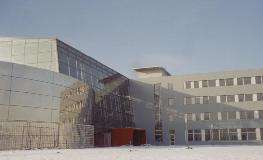
\includegraphics[width=\textwidth]{bilder/garching.jpg}
	\caption{Bild der Mathe und Info Gebäudes in Garching b. München}
	\label{fig:garching}
\end{figure}

Als Beispiel kommen die Worte Grundlagen und Einleitung in den Index \index{Grundlagen} \index{Einleitung}

%%%%%%%%%%%%%%%%%%%%%%%%%%%%%%%%%%%%%%%%%%%%%%%%%%%%%%%%%%%%%%%%%%%%%%%%%%%%%%%
% *** Gleichungen ***
%%%%%%%%%%%%%%%%%%%%%%%%%%%%%%%%%%%%%%%%%%%%%%%%%%%%%%%%%%%%%%%%%%%%%%%%%%%%%%%
%
\section{Gleichungen}\label{sec:gleichungen}
%
Dies ist eine einfache Gleichung
%
\begin{eqnarray}\label{gl:einfache_gleichung}
  y & = & ax^2 + bx + c
\end{eqnarray}

In Abschnitt \ref{sec:gleichungen} erkläre ich den Gleichung \ref{gl:einfache_gleichung} und die ist ganz prima. 


\begin{eqnarray}\label{gl:einfache_gleichung2}
	y & = & ax^2 + bx + c +f
\end{eqnarray}

In Abschnitt \ref{sec:gleichungen} erkläre ich den Gleichung \ref{gl:einfache_gleichung2} und die ist ganz prima. 

\section{Quellcode}
Man kann mit \LaTeX{} super Quelltext oder Snippets setzen. Dazu muss man die Sprache konfigurieren und wie man möchte, dass der Quellcode aussieht. Das kann pro Snippet passieren. . 
\lstset{
	numbers=left, numberstyle=\tiny, numbersep=5pt,
basicstyle=\small, % print whole listing small 
%keywordstyle=\ttb\color{deepblue}
%identifierstyle=, % nothing happens 
%commentstyle=\color{white}, % white comments 
%stringstyle=\ttfamily, % typewriter type for strings 
%showstringspaces=false} % no special string spaces
}
\begin{lstlisting}[columns=fullflexible,showspaces=false,showtabs=false, language=Python, frame=single, caption={Fakultaetsberechnung}]
def factorial(num): 
  if num < 0: 
      print("Factorial of negative num does not exist")
  elif num == 0: 
    return 1
  else: 
  fact = 1
  while(num > 1): 
    fact *= num 
    num -= 1
  return fact 
\end{lstlisting}

\section{Tabellen}
Tabellen sind ebenfalls gleitende Objekte so wie Bilder. 
\begin{table}
	\centering
	\begin{tabular}{c|c}
		\textbf{Spalte 1} & \textbf{Spalte 2} \\
		\hline
		\hline
		Eintrag & Eintrag \\
		\hline
	\end{tabular}
	\caption{Eine Tabelle}
\end{table}

\begin{figure}
	\centering
	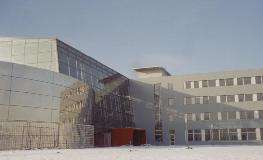
\includegraphics{bilder/garching.jpg}
	\caption[Meine Bacheloranden]{Meine Bacheloranden untereinander im Zoomcall. Meine Bacheloranden untereinander im ZoomcallMeine Bacheloranden untereinander im ZoomcallMeine Bacheloranden untereinander im ZoomcallMeine Bacheloranden untereinander im Zoomcall}
	\label{fig:screenshot}
\end{figure}
\todo{Hier muss ich noch die Beschreibung ergänzen}
\begin{description}
	\item[ Beschreibung] Hier beschreibe ich Hier beschreibe ich Hier beschreibe ich Hier beschreibe ich Hier beschreibe ich Hier beschreibe ich Hier beschreibe ich Hier beschreibe ich Hier beschreibe ich Hier beschreibe ich Hier beschreibe ich Hier beschreibe ich 
	
	\item[ Beschreibung] Hier beschreibe ich Hier beschreibe ich Hier beschreibe ich Hier beschreibe ich Hier beschreibe ich Hier beschreibe ich Hier beschreibe ich Hier beschreibe ich Hier beschreibe ich Hier beschreibe ich Hier beschreibe ich Hier beschreibe ich 
\end{description}
Eine Aufzählung
\begin{itemize}
	\item ein Punkt
	\item noch ein Punkt 
	\begin{itemize}
		\item ein Unterpunkt
	\end{itemize}
	\item ein dritter Punkt
\end{itemize}

\begin{enumerate}
	\item Punkt
	\item Punkt
	\begin{itemize}
		\item bla
		\item blub
	\end{itemize}
	\item Punkt
	\item Punkt
	\begin{enumerate}
		\item weiterer Punkt
		\item noch ein Argument
	\end{enumerate}
	\item Punkt
	
\end{enumerate}
